\chapter{Análisis}
\label{Analisis}

\section{Contexto General en AGESIC}
\label{Analisis:ContextoAgesic}
AGESIC es la agencia encargada de gestionar la plataforma de gobierno electrónico (PGE) del país. Entre los proyectos que componen los servicios electrónicos administrados, se encuentran el “Portal del Estado Uruguayo”, un sistema de expedientes electrónicos y la “Plataforma de Interoperabilidad” (PDI), siendo esta última el objeto de nuestro estudio.

La PDI consta de tres componentes de software principales: La plataforma de middleware, el sistema de seguridad y el sistema de gestión de metadatos \cite{Agesic:GuiaUsos}. La plataforma de middleware tiene el propósito de servir como punto intermedio en la comunicación entre organismos. Todos los servicios registrados por AGESIC son accedidos a través de esta plataforma. El sistema de seguridad permite verificar credenciales y autorizar/desautorizar el acceso a servicios desplegados sobre la plataforma de middleware, así como también la realización de auditorías sobre el acceso. El sistema de gestión de metadatos es una herramienta que almacena información que describe a los servicios en un lenguaje de alto nivel con el fin de aumentar la comprensión sobre la o las funcionalidades provistas por cada servicio.

En la actualidad, no todos los servicios provistos por entes de gobierno forman parte de esta plataforma de interoperabilidad ya que otros entes han desarrollado sus propios ejemplos de esto con anterioridad a la gestión que se realiza hoy en día, aunque gradualmente se está realizando una integración de las mismas. Tal es el caso del Banco de Previsión Social (BPS), ente que con anterioridad a la implantación de la PDI, había desarrollado su propia versión de arquitectura orientada a servicios, intercambiando datos con la Dirección General Impositiva (DGI); en la actualidad, sus servicios se está incorporando progresivamente a la centralización a través de la PDI.
\subsection{Proceso de consumo y publicación de servicios}
\label{Analisis:ProcesoConsumoPublicacion}
Dentro de la plataforma se puede participar tanto publicando servicios como consumiendo (también es posible participar en servicios multi-institucionales \cite{Agesic:GuiaUsos}).

Una definición de proceso para comenzar con la participación en la PDI se encuentra en \cite{Agesic:GuiaUsos} siguiendo un esquema en pasos como los que siguen:
				\begin{enumerate}
				\item Entregar información sobre pautas de uso al ente que pretende hacer uso de la PDI.
				\item Contactar con AGESIC para planificar la ejecución del proyecto de integración.
				\item Actividades de formación y pruebas.
				\item Definir plan de uso en conjunto con AGESIC.
				\item Realizar seguimiento de las pautas establecidas en el primer punto una vez en producción (sea un servicio en producción o una aplicación que consume un servicio existente).
				\end{enumerate}
En base a conversaciones con el cliente, pudimos profundizar sobre estas etapas obteniendo los siguientes casos de uso generales.
\subsubsection{Solicitud para consumir un servicio}	
\label{Analisis:Solicitudparaconsumirunservicio}
Un representante de una entidad de gobierno rellena un formulario disponible con múltiples datos acerca de los motivos de la solicitud. \cite{Agesic:FormularioSolicitudV2.5} El solicitante debe conocer previamente acerca del servicio que requiere. En el documento se deben especificar campos como el nombre del servicio y la entidad responsable. En caso de que no existiera el servicio, AGESIC actúa como intermediario en una solicitud a la entidad considerada responsable de proveer tal servicio para su desarrollo.  Si en cambio, se trata de un servicio existente, se toma la información en base al catálogo disponible –tomando en cuenta aspectos importantes para el desarrollo de un cliente que consuma dicho servicio- y se procede a firmar un acuerdo de intercambio de información entre la entidad solicitante y la proveedora.

Como parte de dicho acuerdo de intercambio, se establece un acuerdo de uso por parte del solicitante, que normalmente implica lo que se conoce como SLA (Service Level Agreement) o “Acuerdo de nivel de servicio” .

Acto seguido, los equipos de desarrollo de la entidad solicitante proceden a trabajar en la producción del software cliente, a lo cual AGESIC brinda un soporte para los aspectos de conectividad, pero no participa de ninguna otra forma más que en asistencia; es una tarea enteramente adjudicada a la entidad solicitante.

Luego de que la pieza de software se encuentra terminada, la entidad puede comenzar a hacer uso de la misma en base a los acuerdos de uso establecidos.

\subsubsection{Solicitud para publicar un servicio}	
\label{Analisis:SolicitudPublicarServicio}
Cuando una entidad de gobierno desea publicar un servicio, ya sea por voluntad propia o ante una necesidad de otro organismo que presentó una solicitud ante AGESIC (el caso más común), el proceso comienza rellenando un formulario para la publicación de servicios en el cual se deben detallar aspectos tanto técnicos como de gestión: personas de contacto, soporte técnico, entre otros. \cite{Agesic:FormularioSolicitudV2.7}
AGESIC no realiza un control acerca del propósito del servicio con motivo de 
categorizarlos independientemente de la entidad encargada, sino que maneja una categorización por organismo: los servicios se agrupan por proveedor y se asume que un proveedor no intentará publicar servicios que cubran aspectos abarcados por otro proveedor. Esto se sustenta en base al marco legal de protección de la información, vigente en el país, el cual prohíbe el intercambio de información entre entidades sin autorización previa \cite{Ley} .

Los servicios deben ser desarrollados en base a un documento de pautas estipuladas por AGESIC. Dicho documento contiene información sobre aspectos técnicos a tener en cuenta para el correcto funcionamiento de un servicio dentro de la plataforma \cite{Agesic:RequerimientosPublicacionServicios}. Al momento de la publicación del servicio en la plataforma, se realiza la verificación de cumplimiento de estas pautas. 

Al momento del despliegue en la plataforma, se considera que el servicio ha sido pasado por los procesos de verificación de calidad adecuados, y que todo está en funcionamiento en el área de TI de la entidad proveedora. Como parte de procedimientos futuros, la entidad proveedora debe establecer un mecanismo de reporte de errores que será utilizado por quienes consuman el servicio. 

El despliegue en la plataforma consiste en configurar una política de autorización que implica hacer disponible al servicio para ser vinculado con otros entes para establecer los intercambios de información. Esto no sucede hasta que una entidad solicita el uso del servicio que se quiere publicar. Por otra parte, se crea un “proxy” del servicio dentro de la plataforma de interoperabilidad el cual estará configurado apropiadamente para comunicar a los consumidores con los servidores proveedores del servicio dispuestos por la entidad publicadora. Como parte de este proceso, se realizan pruebas de integración que verifiquen el correcto funcionamiento de la comunicación con el servicio desde la plataforma, aspectos de seguridad de acceso y aspectos de comunicación hacia los servidores que mantienen al servicio funcionando. Existe un procedimiento definido para realizar dichas pruebas.  

\subsubsection{Mantenimiento y seguimiento de la plataforma}	
\label{Analisis:MantenimientoSeguimientoPlataforma}
AGESIC no participa en el mantenimiento de los aspectos individuales de los servicios, sino que se encarga de las tareas de mantenimiento general de la plataforma de interoperabilidad. Existen procedimientos de comunicación con las entidades consumidoras de servicios a través de la plataforma, quienes son notificados acerca de mantenimientos programados. Normalmente estos se realizan en los horarios en los cuales se dan los picos de uso más bajos, de modo de afectar la operativa de la menor forma posible. Estos horarios se definen en base a la información provista por los solicitantes en los formularios de solicitud, así como también a reportes obtenidos a través de una aplicación encargada de monitorear el uso de los servicios de modo de determinar los horarios más convenientes para las tareas.

En los casos en que las tareas de mantenimiento son llevadas a cabo por los propios entes encargados de los servicios, estos se lo comunican a AGESIC, quien se encargará de notificar a los clientes del servicio en cuestión acerca del mantenimiento programado.

En cuanto al monitoreo de servicios, AGESIC se encarga de verificar el estado activo del servicio mediante una consulta tipo “ping” a la dirección de ruteo establecida en la plataforma de interoperabilidad. No se realizan otras medidas actualmente. 

El cumplimiento de los acuerdos de nivel de servicio, así como también sobre facturación por uso y demás, es responsabilidad de cada entidad. La identificación del cliente que consume un servicio se realiza a través de los mecanismos de autenticación de la plataforma.

\subsubsection{Actores en el proceso}	
\label{Analisis:ActoresDelProceso}
Con respecto a los roles que forman parte de las actividades de AGESIC en cuanto a la gobernanza de arquitecturas orientadas a servicios, encontramos a algunos de los actores típicos de este tipo de proyecto, ocupando lugares dentro de los procesos que se describen en esta realidad.

Los encargados de los servicios del lado de los organismos, toman el rol de Service Custodian (Custodio de servicio). Si bien estos no forman parte del equipo activo en las instalaciones, forman parte del proceso por ser los responsables de uno o más servicios ofrecidos por el organismo.

AGESIC actúa en el rol de Cloud Service Owner (Propietario del servicio en la nube) y Cloud Resource Administrator (Administrador de recursos en la nube), ya que es quien presta parte de la infraestructura necesaria para establecer la comunicación con los servicios; específicamente, se encarga de la infraestructura de la plataforma de middleware. Los organismos disponen de sus actores en estos roles para encargarse de la infraestructura propia.

Participa el rol de Service Administrator (Administrador de servicio) encargándose del funcionamiento de los mismos sobre la plataforma. Este rol es compartido con los organismos ya que aquellos tienen sus propios administradores trabajando en sus instalaciones.

Un Schema Custodian (Custodio de esquema) en AGESIC se encarga de definir esquemas normalizados de metadatos para los servicios, aunque estos existen en carácter de recomendación para los organismos.

Existe un Policy Custodian (Custodio de política) también, quien se encarga de mantener las políticas de seguridad de acceso a la PDI.

Para la recolección de datos acerca de los servicios con motivo de ser utilizados en el descubrimiento (en el catálogo), AGESIC dispone de actores en el rol de Service Registry Custodian (Custodio del registro de servicio), siendo las actividades involucradas compartidas con los organismos ya que estos proveen la mayor parte de la información.

Encargándose de la arquitectura de la PDI y los estándares de seguridad de acceso a la plataforma, encontramos actores en los roles de Enterprise Architect (Arquitecto empresarial) y Enterprise Design Standards Custodian (Custodio de estándares de diseño empresarial) respectivamente.

Por último, actuando en los aspectos más directamente relacionados con la gobernanza de arquitecturas orientadas a servicios, existen hoy en día un SOA Security Specialist (Especialista en seguridad en SOA) encargado de la seguridad de acceso a los servicios, y un SOA Governance Specialist (Especialista en gobernanza en SOA), encargado de dirigir las tareas de gobernanza en SOA en toda de la institución.

Varios de los roles que se consideran dentro de la gobernanza en SOA no están contemplados dentro de AGESIC ya que la misma no participa en todas las actividades relacionadas al diseño y desarrollo de los servicios. 

\section{Estrategia de versionado}
\label{Analisis:EstrategiaVersionado}
La creación de una nueva versión de un servicio surge bajo el pedido de el organismo proveedor a AGESIC. Por esto, se debe realizar una nota formal especificando la necesidad del cambio. 
%************ Comentario de JP****************
%Sabemos algo mas de la nota formal?
Una vez que la nueva versión este terminada y funcionando, AGESIC crea un proxy para la nueva versión en su plataforma \emph{WebSphere Data Power Integration} para que otros organismos puedan consumir el servicio.
\emph{WebSphere Data Power Integration} es una herramienta de integración y conectividad de IBM. AGESIC utiliza la versión {WebSphere DataPower Integration Appliance XI50 (Data Power)}.
Ademas de utilizar esta herramienta, AGESIC utiliza un firewall XML a nivel de aplicación para permitir o negar el acceso del servicio invocado basándose en políticas que tome el Administrador de Políticas de Seguridad.
El mecanismo que tiene AGESIC para realizar un pasaje a producción de una nueva versión de servicio
es crear un nuevo proxy (IP/Puerto) bajo la plataforma (Data Power) que esté apuntando a la nueva versión del servicio.
Ejemplo:
				\begin{enumerate}
				\item 192.168.1.133:6001 	= v1.0
				\item 192.168.1.133:6002 	= v2.0
				\end{enumerate}

      \begin{figure}[h]
        \centering
        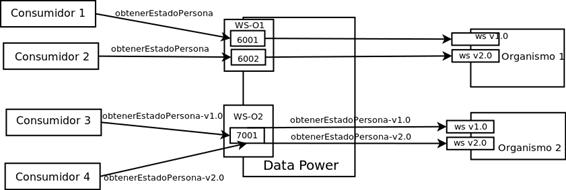
\includegraphics[scale=1]{ej_dataPower}
        \caption{Interacción de servicios con Data Power}
        \label{figura:ej_dataPower}
      \end{figure}
En la figura \ref{figura:ej_dataPower} se ilustra la interacción de los organismos consumidores de un servicio con la plataforma Data Power en base al ejemplo.
Otra alternativa de AGESIC para crear una nueva versión es por intermedio de la plataforma, utilizar el mismo proxy que se está utilizando actualmente pero cambiando el contexto de la URL.
Ejemplo: …/servicios/mides/obtenerEstadoPersona-v2.0 apuntaría a la versión 2.0 del servicio.
%************ Comentario de JP****************
%Yo no entendi mucho como funciona el versionado en Agesic, capaz podes vichar nuevamente esta parte.

La decisión del mantenimiento de las versiones anteriores a la nueva publicada depende del organismo proveedor del servicio. Debe definir si los servicios anteriores estarán disponibles o no para ser consumidos por otros organismos. AGESIC no establece la importancia y condiciones sobre el versionado al momento de la liberación de una nueva versión. Siendo  así muy limitado el mecanismo de publicación de una versión. Hoy solamente se hacen recomendaciones a los organismos pero no se tienen exigencias sobre estos temas.

\section{Calidad de servicios}
\label{Analisis:CalidadServicios}
AGESIC monitorea algunos atributos de calidad y sus valores son ofrecidos en el catalogo de servicios que se describe en la sección \ref{Analisis:CalidadServicios}. Si bien son factores que forman parte de varios modelos de calidad analizados en la sección \ref{MarcoConceptual:calidad}, AGESIC no define ningún modelo de calidad especifico ni establece la forma de evaluar los factores.
La disponibilidad del servicio es uno de los factores de calidad que mide. Por conversaciones con el cliente, la forma de evaluar este factor es realizando ping (invocaciones al endpoint del proveedor) deforma de saber si el servicio esta disponible.
La PDI al utilizar un Middleware como es el ESB, donde los organismos pueden aprovechar los entornos que provee el Middleware de la plataforma para alojar servicios o aplicaciones que requieran infraestructura de hardware o  software avanzada, no disponible por ellos. Esta infraestructura  puede ser necesaria para garantizar determinados niveles de calidad de  servicio en relación, por ejemplo, tiempos de respuesta y disponibilidad \cite{Agesic:GuiaUsos}.
Los productos de ESB de la Plataforma de Middleware proveen mecanismos que pueden ser utilizados por los organismos para el consumo y provisión de servicios. Cuentan con varias funcionalidades nativas que permiten el monitoreo de distintos tipos de información como tiempos de  respuesta de los servicios, contenido de los mensajes, cantidad de  invocaciones a los servicios, etc. En marco de seguridad permite que los organismos deleguen a la PDI la tarea de controlar el acceso a los servicios que proveen.
Todo este conjunto de funcionalidades que ofrecen el ESB son de gran aporte para las mediciones de los atributos de calidad. Pero es inminente la necesidad de establecer que factores son de interés monitorear para los servicios que ofrece la PDI. 
De la manera actual, AGESIC carece de un mecanismo transparente donde permita evaluar de forma directa los niveles de calidad establecidos en el SLA establecido con el proveedor del servicio.

\section{Descubrimientos de Servicios}
\label{Analisis:Catalogo}
AGESIC presenta un catálogo de servicios cuyo mantenimiento es realizado por ellos mismos, y a su vez cuenta con los servicios de una Mesa de Ayuda dedicada a atender requerimientos provenientes de las instituciones públicas usuarias del servicio. Es una motivación de AGESIC poner esta información a disposición de cualquier interesado. El catálogo es de  interés para empresas proveedoras del Estado o cualquier institución, pública o privada, que  desee beneficiarse con el mismo \cite{Agesic:Catalogo}.

El catálogo es accedido a través de una interfaz web disponible en \cite{Agesic:Catalogo} como se ve en la figura \ref{figura:ej_catalogo_agesic} :
      \begin{figure}[h]
        \centering
        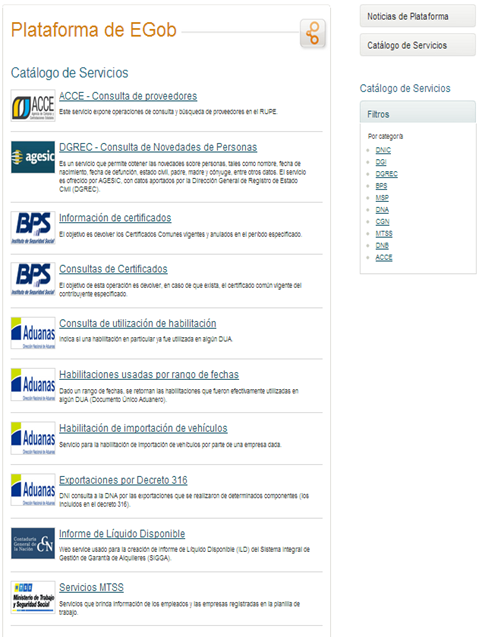
\includegraphics[scale=0.5]{ej_catalogo_agesic}
        \caption{Catalogo de Servicio de AGESIC}
        \label{figura:ej_catalogo_agesic}
      \end{figure}
Cada Web Services cuenta con un conjunto de metadatos sobre el proveedor de servicio: descripción, WSDL, entre otros, y niveles de calidad que se comprometen a cumplir: disponibilidad, tiempos de respuesta, volumen de carga máxima.
      \begin{figure}[h]
        \centering
        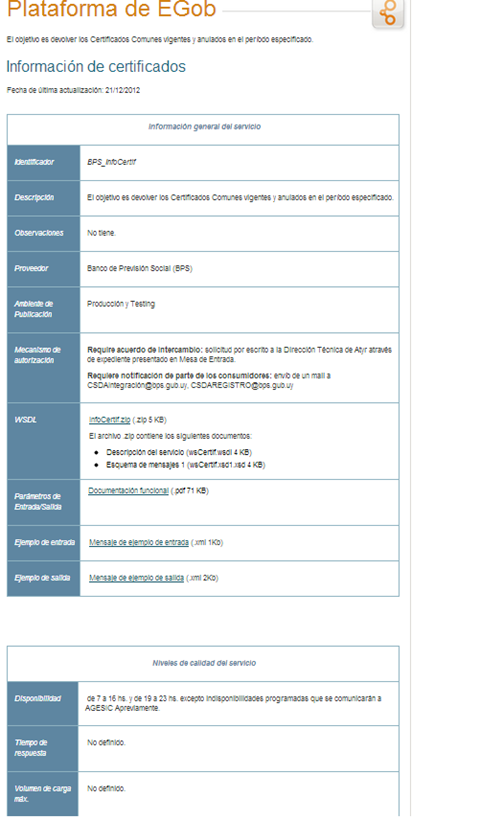
\includegraphics[scale=0.5]{ej_servicio_del_catalogo}
        \caption{Servicio del BPS en el Catalogo de Servicio de AGESIC}
        \label{figura:ej_servicio_del_catalogo}
      \end{figure}
En la figura \ref{figura:ej_servicio_del_catalogo} se puede ver un ejemplo de la información de un servicio que ofrece el catalogo.
A través del catalogo de servicios se realizan el descubren de los servicios publicados. Al visualizar el servicio, no encontramos ninguna información con respecto a las distintas versiones del servicio. De igual manera no ofrece información sobre factores de calidad que permitan asegurar el cumplimiento de los SLA establecidos.

\section{Conclusiones del capitulo}
\label{Analisis:conclusiones}
% Publicacion
\emph{MIG: Falta un resumen de publicación de los servicio}
%Versionado,Calidad y CAtalogo
En cuanto al versionado se toman en cuenta muchas variables a la hora de versionar un servicio pero no está estandarizado este proceso.Hoy solamente se hacen recomendaciones a los organismos pero no se tienen exigencias sobre estos temas. Por lo que es necesario establecer una metodología, debido a la importancia de poder organizar la plataforma. La cantidad de servicios va en aumento, y una buena gestión es fundamental para poder establecer con buenas practicas un proceso de versionado acorde con los cambios que realice el proveedor al servicio. En esta metodología se deben definir la estrategia de versionado. Además de esta elección hay que acondicionar esta estrategia para las necesidades propias, definir cuándo es necesario el pasaje a una nueva versión mayor y cuando no lo es, entre otros aspectos necesarios para la convivencia de múltiples versiones.
Sobre la calidad de los servicios vimos que no existe ningún modelo de calidad definido que permita monitorear los niveles de acuerdo de calidad del servicio en que se compromete ofrecer el proveedor a los clientes de los mismos. Al utilizar un ESB, permite aprovechar muchas funcionalidades que permiten mejorar la calidad y monitorear los servicios. Con una definición de un modelo de calidad, se pueden aprovechar dichas funcionalidades que ofrecen los ESB, brindando información que permitan analizar los rendimientos de los servicios y controlar los criterios de calidad comprometidos por los proveedores.
La información de las distintas versiones existentes de los servicios como el desarrollo en profundidad de los aspectos de calidad de los mismos, no son representadas en el catalogo de servicios que ofrece actualmente AGESIC. El catalogo de servicio es la forma de descubrir lo servicios, por lo que es fundamental poder establecer en el catalogo dicha información para ofrecer a los clientes consumidores del servicio como a los proveedores de los servicios.
